\documentclass[tikz,border=5pt]{standalone}
\usepackage{amsmath}
\usepackage{tikz}
\usetikzlibrary{arrows.meta, angles, quotes}

\begin{document}

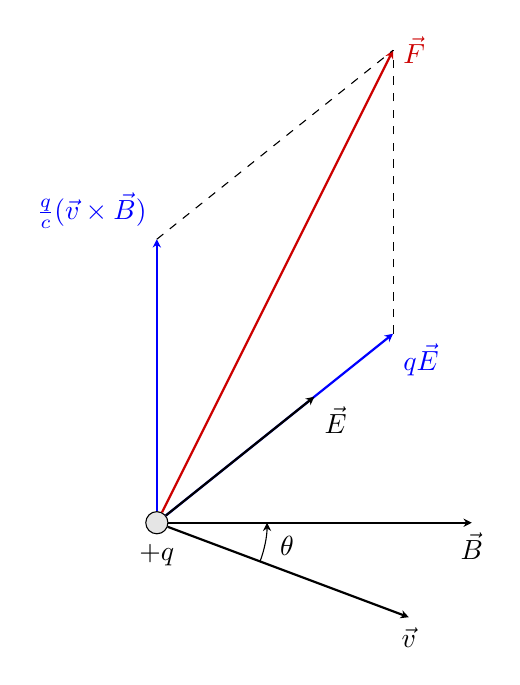
\begin{tikzpicture}[scale=2, 
  >={Stealth[length=3pt,width=3pt]},
  vector/.style={->,thick},
  charge/.style={circle,draw,fill=gray!20,minimum size=8pt,inner sep=0pt}
  ]

% Origin
\node[charge,label=below:{$+q$}] (O) at (0,0) {};
\coordinate (v) at (1.6,-0.6);
\coordinate (B) at (2,0);
\coordinate (Fe) at (1.5,1.2);
\coordinate (E) at (1,0.8);
\coordinate (Fm) at (0,1.8);
\coordinate (F) at (1.5,3);


% Velocity vector v
\draw[vector] (O) -- (v) node[below] {$\vec{v}$};

% Magnetic field B
\draw[vector] (O) -- (B) node[below] {$\vec{B}$};

% qE
\draw[blue,vector] (O) -- (Fe) node[below right] {$q\vec{E}$};

% Electric field E
\draw[vector] (O) -- (E) node[below right] {$\vec{E}$};


% q(v × B)
\draw[blue,vector] (O) -- (Fm) node[above left] {$\frac{q}{c}(\vec{v}\times\vec{B})$};

% Total force F
\draw[red!80!black,vector] (O) -- (F) node[right] {$\vec{F}$};

% Lines
\draw[dashed] (Fm) -- (F);
\draw[dashed] (Fe) -- (F);

% Angle theta between v and B
\pic [draw=black,->,"$\theta$",angle eccentricity=1.2,angle radius=14mm] {angle = v--O--B};

\end{tikzpicture}
\end{document}